\section{Residual Neural Networks}
\label{sec:neural-networks}

Residual neural networks (ResNets) were first introduced in 2016 by \citet{he16} and have their origins in practical application rather than theory.
They are motivated from the fact that in standard deep networks, one can observe deteriorating performance after a certain number of layers has been reached.
An example for this can be seen in \cref{fig:depth-performance-decline} on the left, which depicts the training of a convolutional neural network on the ImageNet classification task \cite{deng09}.
Here, the 34 layer network shows a higher training and validation error than the 18 layer equivalent, which means the worse performance cannot be attributed to overfitting (which is characterized by very low training and high validation error). 
The worse performance of the deeper network is counterintuitive, as models with more layers also have more parameters and hence should be better at learning the given task.
\citet{he16} constructed an easy example which shows that more layers should at least not worsen the results:
Take a trained, shallow network and copy its parameters to the first layers of the deep network.
Set the remaining layers such that they perform an identity mapping, which means they just pass the input through to the next layer.
Then the deep network produces the same output as the shallow one.
This indicates that in general, a deeper network should not yield worse results than one with fewer layers.

Furthermore, deep networks cannot be efficiently replaced by shallow architectures:
Non-flattening theorems state the the number of neurons required by a shallow network, i.e. one with only one hidden layer, grows (almost) exponentially compared to a deep network \cite{lin17,delalleau11}.
An example: the product of $n$ numbers can be computed by a deep network with only $4n$ neurons, where as a flattened equivalent with only one hidden layer would require $2^n$ neurons \cite{lin17}.

\begin{figure}
	\makebox[\textwidth][c]{
		\centering
		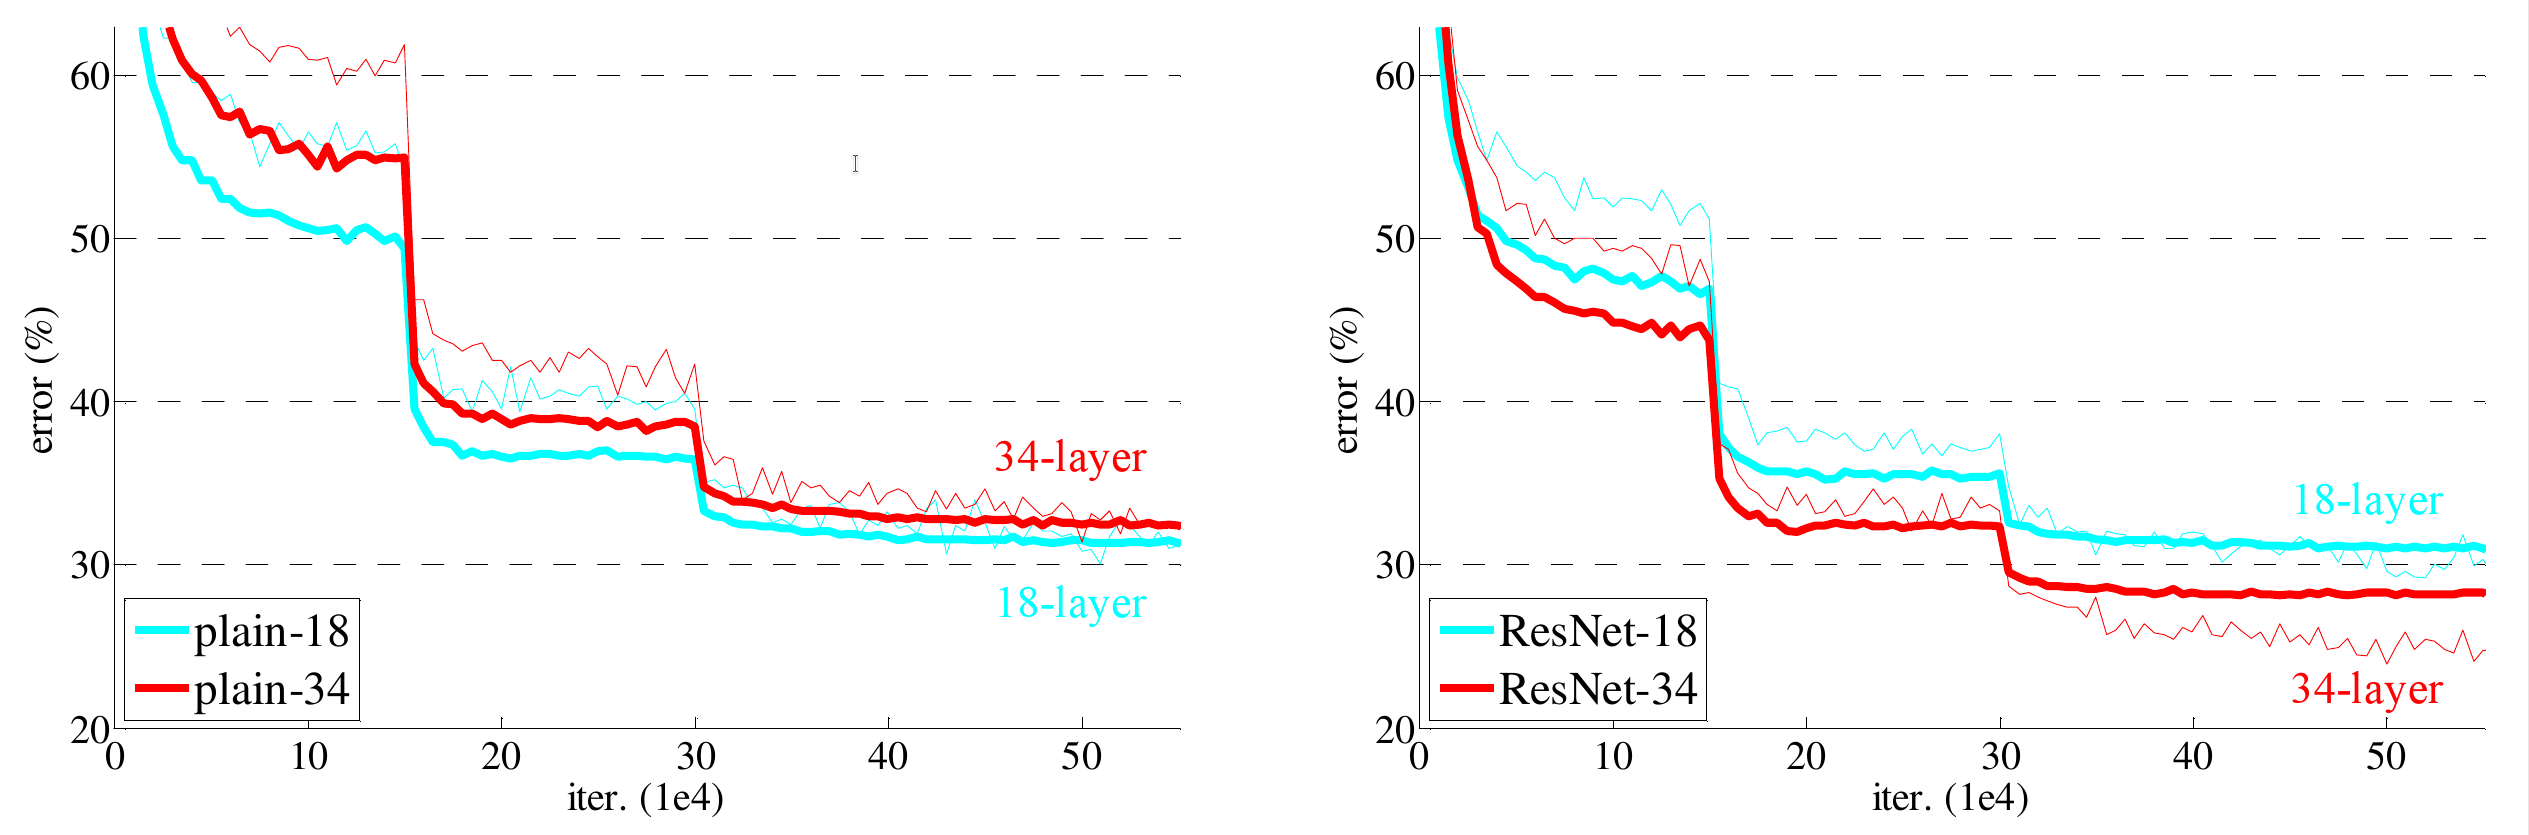
\includegraphics[scale=0.4]{figures/image_net_error_by_kaiming_he.png}
	}
	\caption{
		Training (thin) and validation errors (bold) for a 18- and 34-layer plain network (left) and ResNet (right).
		The plain 34 layer network shows worse results than the 18 layer equivalent, whereas the deeper ResNet performs better than the 18 layer one.
		This is not the case for the plain network.
		This figure originates from the paper "Deep Residual Learning for Image Recognition" by \citet{he16}. \copyright~2016 IEEE.}
	\label{fig:depth-performance-decline}
\end{figure}

%Yet in practice one can observe deteriorating performance after a certain depth has been reached.
%An example for this can be seen in \cref{fig:depth-performance-decline} on the left.
These facts indicate that deeper networks are more efficient and should generally perform better than shallow ones.
Nonetheless, the example in \cref{fig:depth-performance-decline} shows the opposite effect.
It seems that contemporary optimizers are not able to effectively learn the constructed, deeper solution presented above.
\citet{he16} conjecture that this is because it is hard to learn the identity mapping through non-linear layers and suggest that it is easier to learn the zero function instead.
This leads to their proposed network architecture: Residual Neural Networks.

The characteristic feature of ResNets is that they learn residual mappings instead of unreferenced mappings.
Let $f: \cX \rightarrow \cX$ be the function to be approximated by number of (non-linear) layers and $x \in \cX$.
\citet{he16} suggest that instead of learning $f$ directly, to learn the \emph{residual}; given by
\begin{equation}
	\begin{split}
		g: \cX \rightarrow \cX \\
		g(x) \coloneqq f(x) - x \ .
	\end{split}
\end{equation}
This is implemented by creating shortcut connections that skip one or more layers and add the input to the layers' output, resulting in $g(x) + x = f(x)$.
An illustration of a typical residual block is shown in \cref{fig:residual-block}.

\begin{figure}
	\centering
	\begin{tikzpicture}
		[
		font=\scriptsize,
		block/.style ={rectangle, draw=black, thick, text width=15em, align=center, minimum height=1.5em}
		]
		\node[] (a) [block] {Fully Connected Layer (1024)};
		\node[below= -1.5\pgflinewidth of a] (a1) [block] {BatchNorm};
		\node[below= -1.5\pgflinewidth of a1] (b) [block] {ReLU};
		\node[below= 4mm of b] (c) [block] {Fully Connected Layer (1024)};
		\node[below= -1.5\pgflinewidth of c] (c1) [block] {BatchNorm};
		\node[below= -1.5\pgflinewidth of c1] (d) [block] {ReLU};
		\node[below= 4mm of d] (e) [block] {$\bigoplus$};
		\node[above=of a] (x) [] {};
		\draw[->, line width=1pt] (b.south) -- (c.north);
		\draw[->, line width=1pt] (d.south) -- (e.north);
		\draw[->, line width=1pt] (x) -- (a);
		\node[below=of e] (y) [] {};
		\draw[->, line width=1pt] (e) -- (y);
		\node[above=.4 of a] (z) [] {};
		\node[right=12em of z] (h) [] {};
		\draw[line width=1pt] (z.center) -- (h.center);
		\draw[->, bend right, line width=1pt] (h.center) |- (e.east);
	\end{tikzpicture}
	\caption{Typical residual block.
	$\bigoplus$ indicates the inputs of both arrows being summed.
	This particular design was used in \cite{drover18} for 3D Human Pose Estimation.
	Similar blocks are used in image classification and object detection, where the fully connected layers are usually replaced by convolutions.
	}
	\label{fig:residual-block}
\end{figure}

This residual network layout was able to circumvent the decrease in performance that came with an increased number of layers and even showed better results, as one would expect from a model with a greater number of parameters.
Nowadays, ResNets have become an essential part of network architectures and are used in virtually all areas of machine learning, including image classification and object detection \cite{he16,carion20}, semantic segmentation \cite{chen17}, 3D human pose estimation \cite{drover18} and natural language processing \cite{keskar19,conneau16,vaswani17}.
